\section{Analysephase}

\begin{wrapfigure}[11]{r}[0cm]{170px}
	\vspace{-12px}
	\centering
	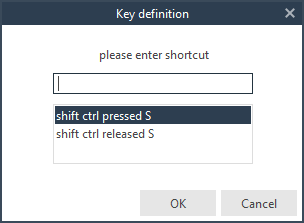
\includegraphics[width=170px]{../graphic/images/screenshots/Alter-Editor}
	\caption{Bestehender Editor}
	\label{fig:existEditor}
\end{wrapfigure}

\subsection{Ist-Analyse}

Seit früheren Versionen existiert bereits ein Editor zur Eingabe von Shortcuts (siehe \autoref{fig:existEditor}). Dieser ist allerdings sehr einfach aufgebaut und beschränkt sich auf die Eingabe eines Shortcuts per Tastatur. Außerdem ist es nicht möglich, Warnungen anzuzeigen oder zwischen bestehenden Shortcuts zu navigieren. Da dieser Editor in keinerlei Hinsicht den gegebenen Anforderungen dieses Projekts entspricht, wurde eine Weiterentwicklung dessen vom Autor als nicht sinnvoll erachtet.

Es wurde bereits ein Datentyp für Shortcuts implementiert. Die allgemeine Definition dafür stellt das Interface \emph{IShortcut} dar. Der Editor sollte sein Ergebnis in Form dieses Datentyps liefern, da \emph{IShortcut} im restlichen System ebenfalls für Tastaturkürzel verwendet wird und somit Konvertierungen vermieden werden können.

\subsection{Sollkonzept}

Der neue Editor muss ebenfalls die Eingabe aber auch die Bearbeitung (z. B. Entfernen einer einzelnen Taste) eines Shortcuts per Tastatur und Maus unterstützen. Für die Navigation und für einen besseren Überblick werden alle bestehenden Tastenkombinationen in tabellarischer Form präsentiert. Es soll zu jedem Zeitpunkt ersichtlich sein, für welche Aktion der Shortcut definiert wird. Eine weitere Anforderung besteht darin, alle Warnungen für die entsprechenden Browser und deren Betriebssysteme anzuzeigen.

\subsection{Anwendungsfälle}

Um eine grobe Übersicht über alle Anwendungsfälle zu erhalten, die von dem umzusetzenden Editor
abgedeckt werden sollen, wurde im Laufe der Analysephase ein Use-Case-Diagramm erstellt. Dieses
Diagramm befindet sich im Anhang \ref{usecase}.

\subsection{\glqq Make or Buy\grqq -Entscheidung}
Am Ende der Analysephase wurde sich die Frage gestellt, ob der Editor selber entwickelt oder gekauft werden soll. Dazu wurde der Markt nach Software durchsucht, welche den Anforderungen dieses Projekts gerecht wird. Da diese Suche zu keinem Ergebnis gekommen war, wurde sich für die eigene Entwicklung des Editors entschieden.

\newpage
